\chapter{Analisi}
\label{chap:analisi}


\section{Scopo del progetto}
La \textit{Web Application} si pone come obiettivo principale, quello di semplificare ed ottimizzare il processo di \textit{onboarding} di flussi logici all'interno di un database. Il raggiungimento di tale obiettivo è subordinato dall'aggiunta di uno strato logico che si colloca sopra le tabelle relazionali presenti all'interno dello \gls{schema} del database, tali tabelle contengono la logica di gestione dei file che devono passare attraverso il \gls{systemintegrator}. Lo strato logico che si vuole creare è suddiviso in 3 stati, questi rappresentano i passaggi che un file compie durante il suo ciclo di vita nel \gls{systemintegrator}. \\
Il primo è lo stato di \textit{retrieve}, in questo stato si definisce se il file in questione viene spedito verso il sistema oppure se il file dev'essere recuperato da un sistema, specificando in ambedue i casi i parametri della macchina esterna che possiede il file. Definita questa fase si presuppone che il file sia già entrato in gestione del \gls{systemintegrator} e dunque avviene la cosiddetta  \textit{routing}, in questa fase vengono definiti i metadati descritti nel paragrafo \ref{subsec:onboarding}, quest'ultimi serviranno per identificare ed eseguire le opportune operazioni sul file. L'ultima fase è la \textit{delivery}, durante questo stadio, bisogna definire come dev'essere spedito il file verso il destinatario.\\
La funzionalità principale richiesta è la creazione di un nuovo flusso logico, esso dunque sarà suddiviso nei 3 stati sopra descritti e ad ogni stato sarà possibile inserire le informazioni necessarie.
Il progetto inoltre, deve dare la possibilità all'utente di registrarsi, scegliendo tra utente normale e  utente amministratore, quest'ultimo ha permessi più elevati, ad esempio modificare informazioni degli altri utenti, eliminare utenti e visualizzare i \gls{log}. \\
Un'ulteriore funzionalità richiesta è la possibilità di utilizzare chiavi di ricerca per visualizzare i flussi presenti ed eventualmente poterli modificare se necessario.
Per aumentare il livello di integrazione con il sistema esistente è richiesta la possibilità di usufruire delle informazioni già presenti internamente al  \gls{systemintegrator}, queste verranno reperite utilizzando le \gls{API} che esso mette a disposizione e saranno selezionabili durante il processo di creazione del flusso.

% \clearpage si o no? vedi formattazione pagina



\section{Attori del sistema}

\begin{itemize}
    \item \textbf{Utente:} è l'utilizzatore generico dell'applicazione, facente parte del team di lavoro \textit{sistemisti file transfer}.  
     \item \textbf{Amministratore:} è colui che oltre ad utilizzare l'applicazione si occupa anche della manutenzione delle utenze e della visualizzazione dei \gls{log} dell'applicazione.
    \item \textbf{IBM®Sterling B2B Integrator:} è il prodotto che utilizzerà i dati inseriti nel database dall'applicazione per la gestione dei file che passano attraverso esso. 
\end{itemize}



\section{Casi d'uso}

In questa sezione verranno descritti i casi d'uso individuati durante le fasi di analisi, ogni caso d’uso ha uno scopo preciso, distinto e univoco. Inizialmente ogni caso d'uso sarà prima descritto utilizzando il formato breve e successivamenge con il formato dettagliato. Infine sarà presente il diagramma \gls{UML} con lo scopo di mostrare graficamente le interazione tra gli attori e i casi d'uso.

\subsection{Casi d'uso formato breve}

\textbf{CUB1-Registrazione}: ogni utente per utilizzare l'applicazione dovrà prima effettuare la registrazione, compilando il form con i dati richiesti e selezionando o meno la voce che indica se l'utente si registra come amministratore.\\
 \\
\textbf{CUB2-Login}: ogni utente registrato per utilizzare l'applicazione dovrà effettuare il login utilizzando le credenziali inserite in fase di registrazione.\\
 \\
\textbf{CUB3-Creazione nuovo flusso}: ogni utente può creare un nuovo flusso logico; per completare la creazione di esso, l'utente dovrà inserire per le 3 fasi: \textit{retrieve}, \textit{routing}, \textit{delivery} tutte le informazioni necessarie.\\
 \\
\textbf{CUB4-Visualizzazione flussi esistenti}: utilizzando delle chiavi di ricerca l'utente può ricercare e visualizzare i flussi presenti.\\
 \\
\textbf{CUB5-Modifica flusso}: ogni utente può effettuare la modifica di un determinato flusso, correggendo le informazioni salvate rispetto ad esso.\\
 \\
\textbf{CUB6-Eliminazione flusso}: ogni utente può eliminare tutte le informazioni riguardati un flusso, rimuovendolo così dal database.\\
 \\
\textbf{CUB7-Gestione utenti}: l'utente amministratore può visualizzare, modificare ed eliminare i dati relativi ad altri utenti.\\
 \\
\textbf{CUB8-Visualizzazione log}: l'utente amministratore può visualizzare la tabella dei \gls{log}, contente in ordine cronologico le azioni compiute dagli utenti che utilizzano l'applicazione.\\
 \\
\textbf{CUB9-Riutilizzo operazioni esistenti}: durante la creazione di un flusso, in particolare durante lo stato di \textit{routing}, l'utente può selezionare ed utilizzare delle operazioni già definite oppure può scegliere di crearne di nuove.
\subsection{Casi d'uso formato dettagliato}

%%%%%%%%%%%%%%%%%%%%%%%%%%%%%%%%%%%%%%%%%%%%%%%%%%%%%%% 1
\textbf{Caso d’uso CUD1:} Registrazione (CUB1) \\
\textbf{Portata:} Applicazione \textit{onboarding} flussi\\
\textbf{Livello:} Obiettivo utente \\
\textbf{Attore primario:} Utente non registrato \\
\textbf{Attore secondario:} Sistema \\
\textbf{Attore finale:} Utente non registrato \\
\textbf{Parti interessate e interessi:}
Utente non registrato, vuole creare una nuova utenza per poter accedere alle funzionalità del sistema.\\
\textbf{Pre-condizioni:} L’utente che vuole registrarsi deve avere una email non ancora associata a
nessun altro account. \\
\textbf{Garanzia di successo:} Il sistema registra i dati relativi all’account creato. L’utente viene
indirizzato alla pagina login dove può effettuare l’accesso tramite le credenziali indicate in fase di registrazione. \\
\textbf{Scenario principale di successo:} 
\begin{enumerate}
  \item L’utente non essendo ancora registrato accede alla pagina di registrazione
  \item L'utente inserisce i dati richiesti, assicurandosi di avere una mail non ancora utilizzata per altre utenze
  \item L'utente seleziona l'opzione utente normale oppure utente amministratore
  \item Il sistema crea l'utenza
  \item L'utente viene indirizzato alla pagina di login 
\end{enumerate} 
\  \\
\textbf{Estensioni(o passaggi alternativi) :}
\begin{enumerate}
 \setcounter{enumi}{1} 
 \item
     \begin{enumerate}
     \item Inserimento mail già in uso
        \begin{enumerate}
            \item Il sistema segnala l’errore e lo notifica all’utente
        \end{enumerate}
     \item Inserimento password non corretto
     \begin{enumerate}
            \item Il sistema segnala l’errore e lo notifica all’utente
        \end{enumerate}
    \end{enumerate}
\end{enumerate}
\clearpage


%%%%%%%%%%%%%%%%%%%%%%%%%%%%%%%%%%%%%%%%%%%%%%%%%%%%%%% 2



\ \\
\textbf{Caso d’uso CUD2:} Login (CUB2) \\
\textbf{Portata:} Applicazione \textit{onboarding} flussi\\
\textbf{Livello:} Obiettivo utente \\
\textbf{Attore primario:} Utente \\
\textbf{Attore secondario:} Sistema \\
\textbf{Attore finale:} Utente \\
\textbf{Parti interessate e interessi:}
Utente registrato, vuole poter accedere all’applicazione tramite le sue credenziali, inserite in fase di
registrazione.\\
\textbf{Pre-condizioni:} L’utente deve aver già effettuato la fase di registrazione al sistema. \\
\textbf{Garanzia di successo:} L'utente viene autenticato dal sistema e viene indirizzato verso la pagina principale dell'applicazione. \\
\textbf{Scenario principale di successo:} 
\begin{enumerate}
  \item L’utente non ha ancora effettuato il login all’applicazione
  \item L’utente inserisce le credenziali del suo account, inserite in fase di registrazione
  \item Il sistema verifica le credenziali
  \item L’utente accede al suo account e viene indirizzato verso la pagina principale dell’applicazione
\end{enumerate} 
\  \\
\textbf{Estensioni(o passaggi alternativi) :}
\begin{enumerate}
 \item
     \begin{enumerate}
     \item L’utente ha già effettuato il login in precedenza senza aver effettuato successivamente un logout
        \begin{enumerate}
            \item L'utente accede automaticamente senza passare dalla schermata di login
        \end{enumerate}
    \end{enumerate}
 \setcounter{enumi}{2}
 \item 
     \begin{enumerate}
     \item L’utente inserisce credenziali non valide
        \begin{enumerate}
            \item Il sistema segnala l’errore e lo notifica all’utente
        \end{enumerate}
    \end{enumerate}
\end{enumerate}
%%%%%%%%%%%%%%%%%%%%%%%%%%%%%%%%%%%%%%%%%%%%%%%%%%%%%%% 3




\ \\
\textbf{Caso d’uso CUD3:} Creazione nuovo flusso (CUB3) \\
\textbf{Portata:} Applicazione \textit{onboarding} flussi\\
\textbf{Livello:} Obiettivo utente \\
\textbf{Attore primario:} Utente \\
\textbf{Attore secondario:} Sistema, IBM®Sterling B2B Integrator \\
\textbf{Attore finale:} Utente \\
\textbf{Parti interessate e interessi:} \\
Utente, vuole poter inserire le informazioni riguardanti al flusso che sta registrando.\\
IBM®Sterling B2B Integrator, attraverso l'utilizzo le API messe a disposizione rende possibile la scelta di alcuni parametri da inserire.\\
\textbf{Pre-condizioni:} L’utente deve aver già effettuato la registrazione all’applicazione ed aver effettuato successivamente il login.\\
\textbf{Garanzia di successo:} L'utente viene guidato dall'applicazione nell'inserimento dei dati necessari per la corretta creazione del flusso. L'inserimento avviene con un messaggio di successo e i dati vengono inviati correttamente al database.
\clearpage
\textbf{Scenario principale di successo:} 
\begin{enumerate}
  \item L’utente entra nella sezione creazione nuovo flusso
  \item L’utente inserisce le informazioni riguardanti alla fase di \textit{retrieve}
    \begin{enumerate}
        \item L'utente specifica che il \gls{systemintegrator} si occuperà del recupero del file
        \item L'utente inserisce i dati riguardati alla macchina esterna al sistema che possiede i file, specificando \gls{ip}, Porta \gls{tcpip} e protocollo di comunicazione
        \item In base al protocollo scelto l'utente dovrà inserire le informazioni richieste da esso per la corretta configurazione
        % , la scelta del protocollo è tra i seguenti: FTP, FTPS, SFTP, HTTP, Connect:Direct, File System.
    \end{enumerate}
  \item L'utente passa all'inserimento delle informazioni riguardanti alla fase di \textit{routing} 
  \begin{enumerate}
      \item L'utente inserisce i metadati riguardanti all'identificazione del flusso, secondo la naming descritta in \ref{subsec:onboarding}
      \item L'utente inserisce il numero e l'ordine delle operazioni che vuole siano effettuate durante questa fase
      \item Per ogni operazione selezionata, l'utente specifica i parametri necessari per l'operazione (cfr. \ref{subsec:cu9})
  \end{enumerate}
  \item L’utente inserisce i dati riguardanti alla fase di \textit{delivery}
  \begin{enumerate}
      \item L'utente specifica il destinatario del file
      \item L'utente visualizza le informazioni riguardanti al destinatario recuperate dal sistema
  \end{enumerate}
  \item Il sistema notifica l'utente del salvataggio corretto del flusso creato
\end{enumerate} 
\  \\
\textbf{Estensioni(o passaggi alternativi) :}
\begin{enumerate}
\setcounter{enumi}{1}
 \item
     \begin{enumerate}
     \item L’utente specifica che il file verrà inviato verso il \gls{systemintegrator}
     \item L'utente inserisce i dati riguardanti al protocollo attraverso il quale il file verrà inviato da parte del mittente
    \end{enumerate}
 
 \item 
     \begin{enumerate}
     \item Il sistema si accorge che l'identificatore del flusso è gia in uso
        \begin{enumerate}
            \item Il sistema segnala l’errore e lo notifica all’utente
        \end{enumerate}
    \end{enumerate}
\setcounter{enumi}{4}    
 \item 
     \begin{enumerate}
     \item Il database verso il quale il sistema è in scrittura non risponde
        \begin{enumerate}
            \item Il sistema segnala l’errore e lo notifica all’utente
        \end{enumerate}
     \item Il sistema si accorge di un errore generico nel flusso
        \begin{enumerate}
            \item Il sistema segnala l’errore e lo notifica all’utente
        \end{enumerate}  
    \end{enumerate}
\end{enumerate}

\clearpage


%%%%%%%%%%%%%%%%%%%%%%%%%%%%%%%%%%%%%%%%%%%%%%%%%%%%%%% 4




\ \\
\textbf{Caso d’uso CUD4:} Visualizzazione flussi esistenti (CUB4) \\
\textbf{Portata:} Applicazione \textit{onboarding} flussi\\
\textbf{Livello:} Obiettivo utente \\
\textbf{Attore primario:} Utente \\
\textbf{Attore secondario:} Sistema \\
\textbf{Attore finale:} Utente \\
\textbf{Parti interessate e interessi:} 
Utente, vuole poter utilizzare chavi di ricerca per visualizzare tutti i flussi che rispettano tale ricerca, ordinare i flussi in ordine alfabetico oppure in ordine cronologico dalla data di creazione. \\
\textbf{Pre-condizioni:} L’utente deve aver già effettuato la registrazione all’applicazione ed aver effettuato successivamente il login.\\
\textbf{Garanzia di successo:} L'utente seleziona le chiavi di ricerca d'interesse, il sistema mostra la lista dei flussi che rispettano la ricerca. I flussi vengono ordinati in base alle richieste dell'utente. \\
\textbf{Scenario principale di successo:} 
\begin{enumerate}
  \item L’utente entra nella sezione visualizzazione flussi
  \item L'utente seleziona le chiavi di ricerca d'interesse
  \item Il sistema mostra il risultato della ricerca
  \item L'utente seleziona un ordinamento su una delle chiavi
  \item Il sistema dispone i flussi secondo il nuovo ordinamento
\end{enumerate} 
\  \\
\textbf{Estensioni(o passaggi alternativi) :}
\begin{enumerate}
\setcounter{enumi}{2}
 \item
     \begin{enumerate}
     \item Non è presente nessun risultato che soddisfa i criteri di ricerca
     \begin{enumerate}
            \item Il sistema notifica l’utente
        \end{enumerate}
    \end{enumerate}
 \end{enumerate} 

%%%%%%%%%%%%%%%%%%%%%%%%%%%%%%%%%%%%%%%%%%%%%%%%%%%%%%% 5


\ \\
\textbf{Caso d’uso CUD5:} Modifica flusso (CUB5) \\
\textbf{Portata:} Applicazione \textit{onboarding} flussi\\
\textbf{Livello:} Obiettivo utente \\
\textbf{Attore primario:} Utente \\
\textbf{Attore secondario:} Sistema \\
\textbf{Attore finale:} Utente \\
\textbf{Parti interessate e interessi:} 
Utente, vuole poter modificare le informazioni riguardanti un flusso. \\
\textbf{Pre-condizioni:} L’utente deve aver effettuato la ricerca del flusso che vuole aggiornare.\\
\textbf{Garanzia di successo:} L'utente modifica dei parametri di un flusso e quest'ultimo viene aggiornato e salvato all'interno del database.
\clearpage
\textbf{Scenario principale di successo:} 
\begin{enumerate}
  \item L'utente seleziona il flusso che ha intenzione di modificare
  \item L'utente modifica i parametri che vuole aggiornare
  \item L'utente salva le modifiche
  \item Il sistema notifica l'utente del corretto aggiornamento del flusso.
\end{enumerate} 
\  \\
\textbf{Estensioni(o passaggi alternativi) :}
\begin{enumerate}
\setcounter{enumi}{3}
 \item
     \begin{enumerate}
     \item Il sistema si accorge di un errore generico nel flusso modificato
     \begin{enumerate}
            \item Il sistema segnala l’errore e lo notifica all’utente
        \end{enumerate}
     \item Il database verso il quale il sistema è in scrittura non risponde
        \begin{enumerate}
            \item Il sistema segnala l’errore e lo notifica all’utente
        \end{enumerate}
    \end{enumerate}
 \end{enumerate} 


%%%%%%%%%%%%%%%%%%%%%%%%%%%%%%%%%%%%%%%%%%%%%%%%%%%%%%% 6
\ \\
\textbf{Caso d’uso CUD6:} Eliminazione flusso (CUB6) \\
\textbf{Portata:} Applicazione \textit{onboarding} flussi\\
\textbf{Livello:} Obiettivo utente \\
\textbf{Attore primario:} Utente \\
\textbf{Attore secondario:} Sistema \\
\textbf{Attore finale:} Utente \\
\textbf{Parti interessate e interessi:} 
Utente, vuole poter eliminare dal database un flusso. \\
\textbf{Pre-condizioni:} L’utente deve aver effettuato la ricerca del flusso che vuole eliminare.\\
\textbf{Garanzia di successo:} L'utente seleziona di voler eliminare un determinato flusso e da la conferma della scelta.\\
\textbf{Scenario principale di successo:} 
\begin{enumerate}
  \item L'utente seleziona il flusso che ha intenzione di eliminare
  \item Il sistema chieda la conferma della scelta
  \item L'utente conferma
  \item Il sistema notifica l'utente della corretta eliminazione del flusso.
\end{enumerate} 
\  \\
\textbf{Estensioni(o passaggi alternativi) :}
\begin{enumerate}
\setcounter{enumi}{2}
\item
    \begin{enumerate}
        \item L'utente annulla la richiesta
        \begin{enumerate}
            \item Il sistema notifica l'utente del corretto annullamento della richiesta
        \end{enumerate}
    \end{enumerate}
 \item
     \begin{enumerate}
     \item Il sistema si accorge di un errore generico nel flusso modificato
     \begin{enumerate}
            \item Il sistema segnala l’errore e lo notifica all’utente
        \end{enumerate}
     \item Il database verso il quale il sistema è in scrittura non risponde
        \begin{enumerate}
            \item Il sistema segnala l’errore e lo notifica all’utente
        \end{enumerate}
    \end{enumerate}
 \end{enumerate} 


%%%%%%%%%%%%%%%%%%%%%%%%%%%%%%%%%%%%%%%%%%%%%%%%%%%%%%% 7
\ \\
\textbf{Caso d’uso CUD7:} Gestione utenti (CUB7) \\
\textbf{Portata:} Applicazione \textit{onboarding} flussi\\
\textbf{Livello:} Obiettivo utente \\
\textbf{Attore primario:} Utente amministratore \\
\textbf{Attore secondario:} Sistema \\
\textbf{Attore finale:} Utente amministratore \\
\textbf{Parti interessate e interessi:} 
Utente amministratore vuole poter modificare, visualizzare ed eliminare gli utenti registrati all'applicazione se necessario.\\
\textbf{Pre-condizioni:} L’utente amministratore dev'essersi autenticato correttamente.\\
\textbf{Garanzia di successo:} L'utente amministratore seleziona l'utente da gestire , apporta le opportune modifiche e salva quest'ultime.\\
\textbf{Scenario principale di successo:} 
\begin{enumerate}
  \item L'amministratore seleziona l'utente da gestire
  \item L'amministratore apporta le opportune modifiche
  \item L'amministratore salva le modifiche
  \item Il sistema notifica l'amministratore del corretto salvataggio delle modifiche
\end{enumerate} 
\  \\
\textbf{Estensioni(o passaggi alternativi) :}
\begin{enumerate}
\setcounter{enumi}{2}
\item
    \begin{enumerate}
        \item L'amministratore annulla la richiesta di modifica
        \begin{enumerate}
            \item Il sistema notifica l'utente del corretto annullamento della richiesta
        \end{enumerate}
    \end{enumerate}
    \begin{enumerate}
        \item Il database verso il quale il sistema è in scrittura non risponde
        \begin{enumerate}
            \item l sistema segnala l’errore e lo notifica all’utente
        \end{enumerate}
    \end{enumerate}
 \end{enumerate} 
 
 %%%%%%%%%%%%%%%%%%%%%%%%%%%%%%%%%%%%%%%%%%%%%%%%%%%%%%% 8
\ \\
\textbf{Caso d’uso CUD8:} Visualizzazione log (CUB8) \\
\textbf{Portata:} Applicazione \textit{onboarding} flussi\\
\textbf{Livello:} Obiettivo utente \\
\textbf{Attore primario:} Utente amministratore \\
\textbf{Attore secondario:} Sistema \\
\textbf{Attore finale:} Utente amministratore \\
\textbf{Parti interessate e interessi:} 
Utente amministratore vuole poter consultare i \gls{log} dell'applicazione suddivisi per giorno.\\
\textbf{Pre-condizioni:} L’utente amministratore dev'essersi autenticato correttamente.\\
\textbf{Garanzia di successo:} L'utente amministratore seleziona un determinato giorno e visualizza correttamente i \gls{log} dell'applicazione.\\
\textbf{Scenario principale di successo:} 
\begin{enumerate}
  \item L'amministratore seleziona il giorno per cui è interessato visualizzare i \gls{log}
  \item Il sistema mostra i dati richiesti
\end{enumerate} 
\  \\
\textbf{Estensioni(o passaggi alternativi) :}
\begin{enumerate}
\item
    \begin{enumerate}
        \item Il giorno richiesto da parte dell'amministratore non è disponibile
        \begin{enumerate}
            \item Il sistema notifica l'amministratore
        \end{enumerate}
    \end{enumerate}
\item
    \begin{enumerate}
        \item Il database verso il quale il sistema è in lettura non risponde
        \begin{enumerate}
            \item l sistema segnala l’errore e lo notifica all’utente
        \end{enumerate}
    \end{enumerate}
 \end{enumerate} 



 %%%%%%%%%%%%%%%%%%%%%%%%%%%%%%%%%%%%%%%%%%%%%%%%%%%%%%% 9
\label{subsec:cu9}
\ \\
\textbf{Caso d’uso CUD9:} Riutilizzo operazioni esistenti (CUB9) \\
\textbf{Portata:} Applicazione \textit{onboarding} flussi\\
\textbf{Livello:} Obiettivo utente \\
\textbf{Attore primario:} Utente\\
\textbf{Attore secondario:} Sistema \\
\textbf{Attore finale:} Utente \\
\textbf{Parti interessate e interessi:} 
Utente, durante la fase di \textit{routing} vuole poter riutilizzare le operazioni definite precedentemente. \\
\textbf{Pre-condizioni:} L’utente ha compilato correttamente i dati della fase di \textit{retrieve}. Nel sistema è presente almeno un'operaziona già salvata. \\
\textbf{Garanzia di successo:} L'utente seleziona un'operazione già salvata precedentemente e la utilizza per il flusso in questione.\\
\textbf{Scenario principale di successo:} 
\begin{enumerate}
  \item L'utente seleziona una tipologia di operazione per la fase di \textit{routing}
  \item Il sistema mostra le operazioni esistenti per la tipologia selezionata
  \item L'utente seleziona una delle operazioni esistenti
  \item Il sistema mostra la configurazione dell'operazione selezionata
  \item L'utente ripete i passi [1-4] da 0 al numero di operazioni necessarie da effettuare per il flusso
\end{enumerate} 
\  \\
\textbf{Estensioni(o passaggi alternativi) :}
\begin{enumerate}
\setcounter{enumi}{1}
\item
    \begin{enumerate}
        \item Non sono presenti operazioni già esistenti per la tipologia di operazione selezionata
        \begin{enumerate}
            \item Il sistema notifica l'utente e permette a quest'ultimo di creare una nuova operazione
        \end{enumerate}
    \end{enumerate}
\setcounter{enumi}{3}
\item
    \begin{enumerate}
        \item L'utente modifica un parametro della configurazione dell'operazione esistente
        \begin{enumerate}
            \item Il sistema crea una nuova configurazione e lascia intatta l'operazione esistente selezionata in precedenza
        \end{enumerate}
    \end{enumerate}
 \end{enumerate} 

\clearpage

\subsection{Diagramma dei casi d'uso}
Questo diagramma è una rappresentazione dei requisiti funzionali del sistema, dei servizi offerti da esso e delle interazioni che gli attori hanno con il sistema stesso. \\

\ \\
\begin{figure}
\begin{center}
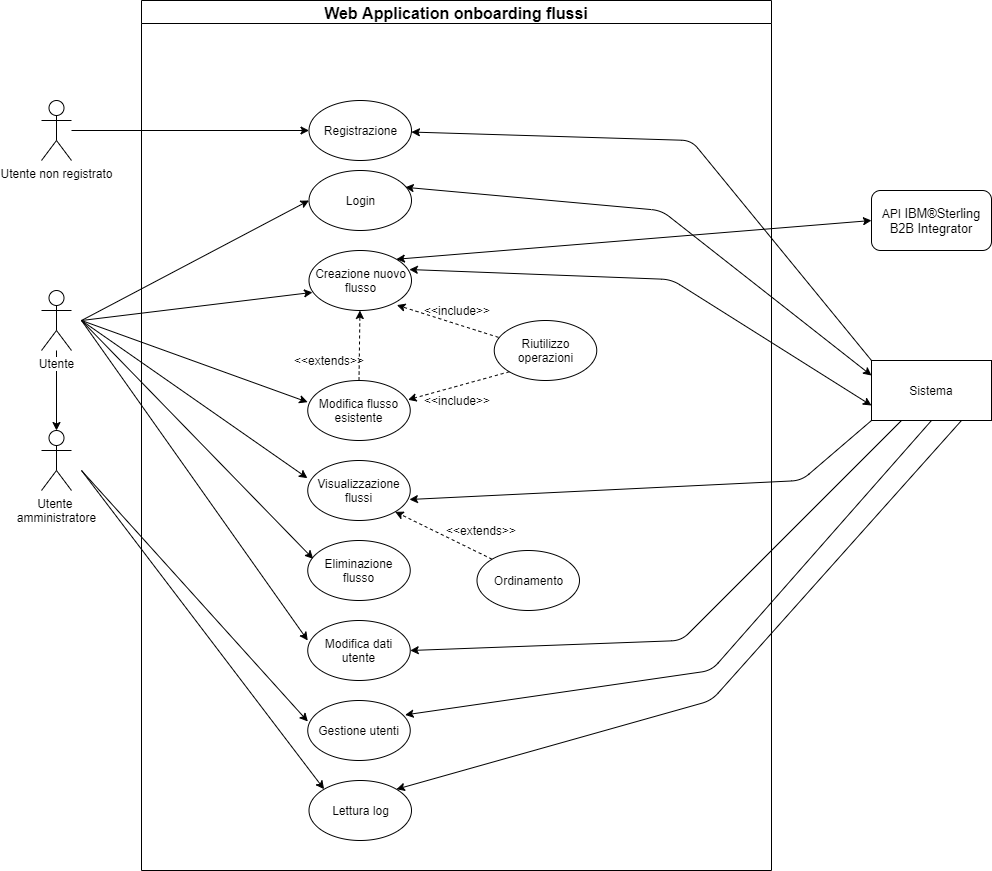
\includegraphics[width=1.0\columnwidth]{images/diagramma_casi_d_uso.png}
\end{center}
\caption{Diagramma dei casi d'uso}
\label{fig:casiuso}
\end{figure}


\clearpage
\subsection{Definizione requisiti}
Di seguito verrà mostrata la classificazione utilizzata per il tracciamento dei requisiti richiesti in realzione ai casi d'uso che li soddisfano: 
\begin{center}
    \textbf{R [ Tipo ][ Priorità ]-[ Codice ]}
\end{center}
dove il significato di ogni parametro della classificazione è esposto di seguito.
\begin{itemize}
    \item \textbf{Tipo:} Funzionale, di qualità, di vincolo
    \begin{itemize}
        \item \textbf{F:} Requisito funzionale. Questi requisiti definiscono una funzionalità del sistema software, in termini di servizi che esso deve fornire, definendone la tipologia degli ingressi e delle uscite, nonché il comportamento;
        \item \textbf{Q:} Requisito di qualità. Includono requsiti di correttezza, affidabilità, robustezza, efficienza ed usabilità del sistema software;
        \item \textbf{V:} Requisito di vincolo. Rappresenta una limitazione tecnologica o strategica;
    \end{itemize}
    \item \textbf{Priorità:} Obbligatorio, Desiderabile, Opzionale  
    \begin{itemize}
        \item \textbf{O:} obbligatorio, indica un requisito irrinunciabile per il committente;
        \item \textbf{D:} requisito desiderabile, ma non strettamente necessario;
        \item \textbf{Z:} opzionale, facoltativo. Verrà soddisfatto solo al
completamento di tutti gli altri obiettivi.
    \end{itemize}
    \item \textbf{Codice:} codice numerico identificativo del requisito. È costituito da uno o più numeri
interi positivi separati da punti, opportunamente ordinati in maniera gerarchica, nel formato
X.Y.Z.  
\end{itemize}

\ \\
Nella tabella qui di seguito (\ref{tab:funz}) verranno riassunti i requisiti funzionali e i casi d'uso ad essi associati. 

%%%%%%%%%%%%%%%%%%%%%%%%%%%%%%%%%%TABELLE
%%%%%%%%%%%%%%%%%%%%%%%%%%%%%%%%%% Funzionali
\begin{longtable}[c]{|c|l|c|}
\hline
\rowcolor[HTML]{EFEFEF} 
\textbf{Requisito} & \multicolumn{1}{c|}{\cellcolor[HTML]{EFEFEF}\textbf{Descrizione}} & \textbf{Caso d'uso} \\ \hline
\endhead
%
\textbf{RFO-1} & \begin{tabular}[c]{@{}l@{}}L’utente non registrato deve poter registrarsi, inserendo \\
le informazioni obbligatorie richieste.\end{tabular} & CUD1 \\ \hline
\textbf{RFO-2} & \begin{tabular}[c]{@{}l@{}}L'utente non registrato deve poter scegliere di registrarsi \\
come utente normale oppure amministratore.\end{tabular} & CUD1 \\ \hline
\textbf{RFO-3} & \begin{tabular}[c]{@{}l@{}}L'utente deve poter effettuare il login per accedere alla \\applicazione.\end{tabular} & CUD2 \\ \hline
\textbf{RFO-4} &  \begin{tabular}[c]{@{}l@{}}L'utente deve poter inserire le informazioni richieste \\
per la fase di \textit{retrieve}.\end{tabular}& CUD3 \\ \hline
\textbf{RFO-5} & \begin{tabular}[c]{@{}l@{}}L'utente deve poter inserire le informazioni richieste \\
per la fase di \textit{routing}.\end{tabular} & CUD3 \\ \hline
\textbf{RFO-6} & \begin{tabular}[c]{@{}l@{}}L'utente deve poter selezionare tutte le operazioni \\ necessarie per la fase di \textit{routing}.\end{tabular} & CUD3 \\ \hline
\textbf{RFO-7} & \begin{tabular}[c]{@{}l@{}}L'utente deve poter inserire nuove operazioni durante \\la fase di \textit{routing}.\end{tabular} & CUD3 \\ \hline
\textbf{RFO-8} & \begin{tabular}[c]{@{}l@{}}L'utente deve poter inserire le informazioni richieste \\
per la fase di \textit{delivery}.\end{tabular} & CUD3 \\ \hline
\textbf{RFO-9} & \begin{tabular}[c]{@{}l@{}}L'utente deve poter visualizzare le informazioni riguar-\\danti il destinatario durante nella fase di \textit{delivery}.\end{tabular} & CUD3 \\ \hline
\textbf{RFO-10} & \begin{tabular}[c]{@{}l@{}}L'utente deve poter selezionare i parametri recuperati \\ dalle \gls{API} del sistema.\end{tabular} & CUD3 \\ \hline
\textbf{RFO-11} & \begin{tabular}[c]{@{}l@{}}L'utente deve poter utilizzare delle chiavi di ricerca \\ 
per poter visualizzare i flussi salvati.\end{tabular} & CUD4 \\ \hline
\textbf{RFO-12} & \begin{tabular}[c]{@{}l@{}}L'utente deve poter selezionare e modificare i parametri \\ di un determinato flusso.\end{tabular} & CUD5 \\ \hline
\textbf{RFO-13} & \begin{tabular}[c]{@{}l@{}}L’utente deve poter selezionare ed eliminare un \\
determinato flusso.\end{tabular} & CUD6 \\ \hline
\textbf{RFO-14} & \begin{tabular}[c]{@{}l@{}}L’amministratore deve poter visualizzare le informazioni \\
degli altri utenti.\end{tabular} & CUD7 \\ \hline
\textbf{RFO-15} & \begin{tabular}[c]{@{}l@{}}L’amministratore deve poter modificare le informazioni \\
degli altri utenti.\end{tabular} & CUD7 \\ \hline
\textbf{RFO-16} & \begin{tabular}[c]{@{}l@{}}L’amministratore deve poter eliminare altre utenze.\end{tabular} & CUD7 \\ \hline
\textbf{RFO-17} & \begin{tabular}[c]{@{}l@{}}L’amministratore deve poter scegliere di visualizzare i \gls{log}\\ dell'applicazione relativi ad una giornata.\end{tabular} & CUD8 \\ \hline
\textbf{RFO-18} & \begin{tabular}[c]{@{}l@{}}L'utente deve poter riutilizzare le operazioni già definite\\  precedentemente durante la fase di \textit{routing}.\end{tabular} & CUD9 \\ \hline
\caption{Tabella requisiti funzionali}
\label{tab:funz}
\end{longtable}


%%%%%%%%%%%%%%%%%%%%%%%%%%%%%%%%%% Qualità
\ \\
Nella tabella sottostante (\ref{tab:qualita}) verranno riassunti i requisiti qualitativi e i casi d'uso ad essi associati.
\begin{longtable}[c]{|c|l|c|}
\hline
\rowcolor[HTML]{EFEFEF} 
\textbf{Requisito} & \multicolumn{1}{c|}{\cellcolor[HTML]{EFEFEF}\textbf{Descrizione}} & \textbf{Caso d'uso} \\ \hline
\endhead
%
\textbf{RQO-1} & \begin{tabular}[c]{@{}l@{}} Durante l'utilizzo dell'applicazione il sistema notifica l'u-\\
te con feedback costanti\end{tabular} & - \\ \hline
\textbf{RQO-2} & \begin{tabular}[c]{@{}l@{}} Il salvataggio delle password degli utenti all'interno del\\ database è criptato.\end{tabular} & CUD1 \\ \hline
\textbf{RQO-3} & \begin{tabular}[c]{@{}l@{}} L'interfaccia grafica dell'applicazione dev'essere \\ semplice ed intuitiva.\end{tabular} & - \\ \hline
\textbf{RQO-4} & \begin{tabular}[c]{@{}l@{}} L'interfaccia grafica dell'applicazione deve utilizzare i \\
colori principali del logo dell'azienda committente.\end{tabular} & - \\ \hline
\textbf{RQO-5} & \begin{tabular}[c]{@{}l@{}} Il riperimento delle informazioni attraverso l'utilizzo \\ delle \gls{API} messe a disposizione dal sistema dev'essere\\ 
ragionevolmente veloce.\end{tabular} & CUD3 \\ \hline
\textbf{RQD-6} & \begin{tabular}[c]{@{}l@{}} L'utente deve poter selezionare le operazioni che vuole\\
utilizzare attraverso una funzione di tipo \textit{"drag-and-drop"}.\end{tabular} & CUD3 \\ \hline
\textbf{RQO-7} & \begin{tabular}[c]{@{}l@{}} L'utente deve poter ordinare la visualizzazione dei flussi \\
di una ricerca  in ordine alfabetico.\end{tabular} & CUD4 \\ \hline
\textbf{RQD-8} & \begin{tabular}[c]{@{}l@{}} L'utente deve poter ordinare la visualizzazione dei flussi \\
di una ricerca  in ordine cronologico dalla data di crea-\\zione.\end{tabular} & CUD4 \\ \hline
\textbf{RQZ-9} & \begin{tabular}[c]{@{}l@{}} L'inserimento dei \gls{log} nella tabella opportuna del \\database  dev'essere minimale.\end{tabular} & CUD8 \\ \hline
\caption{Tabella requisiti qualitativi}
\label{tab:qualita}
\end{longtable}

%%%%%%%%%%%%%%%%%%%%%%%%%%%%%%%%%% Vincoli
\ \\
Nella tabella sottostante (\ref{tab:vincoli}) verranno riassunti i requisiti di vincolo e i casi d'uso ad essi associati.
\begin{longtable}[c]{|c|l|c|}
\hline
\rowcolor[HTML]{EFEFEF} 
\textbf{Requisito} & \multicolumn{1}{c|}{\cellcolor[HTML]{EFEFEF}\textbf{Descrizione}} & \textbf{Caso d'uso} \\ \hline
\endhead
%
\textbf{RVO-1} & \begin{tabular}[c]{@{}l@{}}L'installazione dell'applicazione deve avvenire su 
entrambi \\ i nodi dell'architettura esistente. \end{tabular} & - \\ \hline
\textbf{RVO-2} & \begin{tabular}[c]{@{}l@{}}L’applicativo deve essere realizzato tramite il \gls{framework}\\
Angular in versione almeno 8. \end{tabular} & - \\ \hline
\textbf{RVO-3} & \begin{tabular}[c]{@{}l@{}}L’applicativo deve essere realizzato tramite il \gls{framework}\\
Spring.\end{tabular} & - \\ \hline
\textbf{RVO-4} & \begin{tabular}[c]{@{}l@{}}L’applicativo deve essere realizzato con l’ausilio della\\
libreria Bootstrap. \end{tabular} & - \\ \hline
\textbf{RVO-5} & \begin{tabular}[c]{@{}l@{}}Il \gls{DBMS} sul quale l'applicazione deve lavorare è Oracle. \end{tabular} & - \\ \hline

\caption{Tabella requisiti di vincolo}
\label{tab:vincoli}
\end{longtable}